\chapter{Results}

The main goal of this analysis was to quantify key metrics of the performance of LGAD sensors. In particular, we analysed the collected charge, the time resolution and the efficiency at the temperature of \qty{-30}{\degreeCelsius}, which will be the temperature of the detector in operation. We compared the results between unirradiated and differently irradiated sensors to test whether the requirements at start and end of life were satisfied. The sensors were also studied at angles between \qty{0}{\degree} and \qty{14}{\degree} relative to the beam direction, in line with the HGTD's expected pseudorapidity coverage: between \(2.4\) and \(4\), which corresponds to an incident angle of \qtyrange{2}{10}{\degree}.

Additionally, some other properties and effects that arose during the analysis were also investigated. Such as, signal coming from neighbouring pads, noise coming from outside the gain layer of the pads, interactions between adjacent pads, and properties of the region lying between two adjacent pads. Certain anomalies were also successfully explained, and the root cause was found in the incorrect voltage range set on an oscilloscope, which caused pulses to be "clipped" below a specific threshold. Moreover, due to a temporary malfunction of the cooling box, one batch of data showed neatly the sensitivity of LGADs to temperature variations.

\section{Main Results}

\begin{figure}[h!tbp]
    \centering
    \includegraphics[width=.9\linewidth]{Images/Results/Irradiated/IME_voltage_charge_.png}
    \captionsetup{width=\captionwidth}
    \caption{Overview of voltage vs collected charge for all the studied sensors from IME. \(\Phi\) is the radiation dose of each sensor in neutron-equivalent fluence.}
    \label{fig:irradiated_IME_voltage_charge}
\end{figure}


\begin{figure}[h!tbp]
    \centering
    \includegraphics[width=.9\linewidth]{Images/Results/Irradiated/IME_voltage_time_resolution_.png}
    \captionsetup{width=\captionwidth}
    \caption{Overview of voltage vs time resolution.}
    \label{fig:irradiated_IME_voltage_time_res}
\end{figure}

The most important properties of the sensors are:

\begin{itemize}
    \item Collected change: the most probable value (MPV) of the Landau*Gaussian convolution (\ref{sec:methods_collected_charge}).
    \item Time resolution: the spread of the Gaussian distribution of the Time of Arrivals (\ref{sec:methods_time_resolution}).
    \item Efficiency: the fraction of incident particles that produce a detectable signal in the sensor. (\ref{sec:methods_efficiency}).
\end{itemize}

Overall all sensors behaved as expected: their collected charge increased with higher bias voltage and decreased with higher radiation dose (fluence), and most of them satisfied the HGTD's requirements.

\subsection{Irradiated}

\subsubsection{IME}

The sensors in the IME group were further split depending on versions and types, to enable more meaningful comparisons between devices with similar characteristics. More specifically:

\begin{itemize}
    \item IMEv3-W12: 2\(\times\)2 array unirradiated, 1\(\times\)3 array unirradiated and 2\(\times\)2 array at \qty{1.5e15}{\neutroneq}.
    \item IMEv2-W7: single pad at \qty{1e14}{\neutroneq} and single pad at \qty{6.5e14}{\neutroneq}.
    \item IMEv3-W16: single pad at \qty{8e14}{\neutroneq} and single pad at \qty{2.5e15}{\neutroneq}.
\end{itemize}

%%% IMEv3-W12, 0 and 
\begin{figure}[h!tbp]
    \centering
    \subfloat[Voltage vs Charge.]{
        \includegraphics[width=.49\linewidth]{Images/Results/Irradiated/IMEv3-W12_voltage_charge_irradiated.png}
        \label{fig:IMEv3-W12_voltage_charge}}
    \hfill
    \subfloat[Voltage vs Time resolution]{
        \includegraphics[width=.47\linewidth]{Images/Results/Irradiated/IMEv3-W12_voltage_time_resolution_irradiated.png}
        \label{fig:IMEv3-W12_voltage_time_res}}
    \vfill
    \subfloat[Voltage vs Efficiency]{
        \includegraphics[width=.47\linewidth]{Images/Results/Irradiated/IMEv3-W12_voltage_efficiency_irradiated.png}
        \label{fig:IMEv3-W12_voltage_efficiency}}
    \captionsetup{width=\captionwidth}
    \caption{IMEv3-W12. The non irradiated sensors (both the 2\(\times\)2 array and the 1\(\times\)3 array) had sufficiently high collected charge at all tested bias voltages, while the time resolution was just short of the \qty{35}{\pico\second} target in the case of the 2\(\times\)2 array, although this is likely to be solved with higher applied voltage. The lack of data for higher voltages was due to erroneous batches. It should be noted that the two pads of the 1\(\times\)3 array had significant and consistent discrepancies in charge and time resolution, presumably due to manufacturing differences. The sensors at \qty{1.5e15}{\neutroneq} had very good performance overall and reached the target time resolution of the beginning of operations at \(\simeq60\%\) of the total expected dose. The efficiency was well above the \(95\%\) goal in all examined batches.}
\end{figure}

\begin{figure}[p!htb]
    \centering
    \subfloat[Voltage vs Charge]{
        \includegraphics[width=.47\linewidth]{Images/Results/Irradiated/IMEv2-W7_voltage_charge_irradiated.png}
        \label{fig:IMEv2-W7_voltage_charge}}
    \hfill
    \subfloat[Voltage vs Time resolution]{
        \includegraphics[width=.45\linewidth]{Images/Results/Irradiated/IMEv2-W7_voltage_time_resolution_irradiated.png}
        \label{fig:IMEv2-W7_voltage_time_res}}
    \vfill
    \begin{minipage}[c]{.47\linewidth}
    \subfloat[Voltage vs Efficiency]{
        \includegraphics[width=.95\linewidth]{Images/Results/Irradiated/IMEv2-W7_voltage_efficiency_irradiated.png}
        \label{fig:IMEv2-W7_voltage_efficiency}}
        % \captionsetup{width=\captionwidth}
    \end{minipage}
    \hfill
    \begin{minipage}[c]{.5\linewidth}
        \captionof{figure}{IMEv2-W7. For both fluences (\qty{1e14}{\neutroneq} and \qty{6.5e14}{\neutroneq}, i.e. low fluence) charge and time resolution were within the targets for larger voltages. Furthermore, the more heavily irradiated sensor, showed a significant variation in the efficiency, which increased from \(\simeq96\%\) up to \(\simeq99\%\).}
\end{minipage}
\end{figure}

\begin{figure}[p!htb]
    \centering
    \subfloat[Voltage vs Charge]{
        \includegraphics[width=.47\linewidth]{Images/Results/Irradiated/IMEv3-W16_voltage_charge_irradiated.png}
        \label{fig:IMEv3-W16_voltage_charge}}
    \hfill
    \subfloat[Voltage vs Time resolution]{
        \includegraphics[width=.45\linewidth]{Images/Results/Irradiated/IMEv3-W16_voltage_time_resolution_irradiated.png}
        \label{figIMEv3-W16_voltage_time_res}}
    \vfill
    \begin{minipage}[c]{.47\linewidth}
    \subfloat[Voltage vs Efficiency]{
        \includegraphics[width=.95\linewidth]{Images/Results/Irradiated/IMEv3-W16_voltage_efficiency_irradiated.png}
        \label{fig:IMEv3-W16_voltage_efficiency}}
    \end{minipage}
    \hfill
    \begin{minipage}[c]{.5\linewidth}
    \captionof{figure}{IMEv3-W16. The sensor at \qty{8e14}{\neutroneq} performed well overall, except for the batch at highest bias voltage, which saw a small but unexpected worsening of time resolution and efficiency. We investigated further the cause of this data but were unable to pinpoint the exact source. The sensor at \qty{2.5e15}{\neutroneq}, corresponding to the end-of-life radiation dose, had a collected charge below the requirements, slightly below \qty{3}{\femto\coulomb}, but it showed satisfactory time resolution and efficiency.}
\end{minipage}
\end{figure}

\subsubsection{USTC}

The data from the USTC sensor was the most affected by missing and erroneous batches, as the data from the irradiated sensor was not available.

\begin{figure}[h!tbp]
    \centering
    \subfloat[Voltage vs Charge]{
        \includegraphics[width=.47\linewidth]{Images/Results/Irradiated/USTC_voltage_charge_.png}
        \label{fig:USTC_voltage_charge}}
    \hfill
    \subfloat[Voltage vs Time resolution]{
        \includegraphics[width=.45\linewidth]{Images/Results/Irradiated/USTC_voltage_time_resolution_.png}
        \label{fig:USTC_voltage_time_res}}
    \vfill
    \begin{minipage}[c]{.47\linewidth}
    \subfloat[Voltage vs Efficiency]{
        \includegraphics[width=.95\linewidth]{Images/Results/Irradiated/USTC_voltage_efficiency_.png}
        \label{fig:USTC_voltage_efficiency}}
    \end{minipage}
    \hfill
    \begin{minipage}[c]{.5\linewidth}
        \captionof{figure}{USTC. The sensor had very good collected charge and efficiency, albeit falling short of the time resolutio aim. It also manifested evident differencies between the two neighbouring pads. Unfortunately, the data of the irradiated USTC sensor was not available, so no comparison was possible.}
\end{minipage}
\end{figure}

\subsubsection{CNM}

The unirradiated sensors were used to measure the time resolution of the MCP (Section \ref{sec:MCP_description}). They had already been tested before (as in \cite{Allaire:2018bof}) and they showed similar performance, with gain up to \qtyrange{40}{50}{}, and time resolution better than \qty{30}{\pico\second}. In this test beam they were also tested irradiated at two fluences: \qty{1.5e15}{\neutroneq} and \qty{2.5e15}{\neutroneq}.

\begin{figure}[h!tbp]
    \centering
    \subfloat[Voltage vs Charge]{
        \includegraphics[width=.47\linewidth]{Images/Results/Irradiated/CNM_voltage_charge_.png}
        \label{fig:CNM_voltage_charge}}
    \hfill
    \subfloat[Voltage vs Time resolution]{
        \includegraphics[width=.45\linewidth]{Images/Results/Irradiated/CNM_voltage_time_resolution_.png}
        \label{fig:CNM_voltage_time_res}}
    \vfill
    \begin{minipage}[c]{.47\linewidth}
    \subfloat[Voltage vs Efficiency]{
        \includegraphics[width=.95\linewidth]{Images/Results/Irradiated/CNM_voltage_efficiency_.png}
        \label{fig:CNM_voltage_efficiency}}
    \end{minipage}
    \hfill
    \begin{minipage}[c]{.5\linewidth}
        \captionof{figure}{CNM. The unirradiated confirmed the good performance of the sensors. At the highest expected radiation dose the sensor had an unexpected counter trend of time resolutio, however, the two batches at lower voltages had a significantly lower amount of data available, potentially underestimating the error on the fit.}
\end{minipage}
\end{figure}

% \FloatBarrier 

\subsection{Angled}

The sensors were studied with incident angle of \qtyrange{0}{14}{\degree}, typically \qty{0}{\degree}, \qty{6}{\degree} and \qty{14}{\degree}. However, due to some missing or erroneous batches or mismatched voltages and angles, not all data points were available.
%%% TODO: more introduction on the angle part?
% \marginpar{\flushleft Maybe more introduction}

\subsubsection{IME}

%%% IMEv3-W12 2x2 100V
\begin{figure}[h!tbp]
    \centering
    \subfloat[Angle vs Charge]{
        \includegraphics[width=.47\linewidth]{Images/Results/angled/IMEv3-W12_angle_charge_-100V.png}
        \label{fig:IMEv3-W12_angle_charge_100V}}
    \hfill
    \subfloat[Angle vs Time resolution]{
        \includegraphics[width=.45\linewidth]{Images/Results/angled/IMEv3-W12_angle_time_resolution_-100V.png}
        \label{fig:IMEv3-W12_angle_time_res_100V}}
    \vfill
    \begin{minipage}[c]{.47\linewidth}
        \subfloat[Angle vs Efficiency]{
            \includegraphics[width=.95\linewidth]{Images/Results/angled/IMEv3-W12_angle_efficiency_-100V.png}
            \label{fig:IMEv3-W12_angle_efficiency_100V}}
    \end{minipage}
    \hfill
    \begin{minipage}[c]{.5\linewidth}
        \captionof{figure}{IMEv3-W12, 2\(\times\)2 array, at \qty{-100}{\volt}. The impact of the angle was small, although it showed an improvement in collected charge and time resolution, as expected.}
\end{minipage}

\end{figure}

%%% IMEv3-W12 1x3 125V
\begin{figure}[h!tbp]
    \centering
    \subfloat[Angle vs Charge]{
        \includegraphics[width=.47\linewidth]{Images/Results/angled/IMEv3-W12_angle_charge_-125V.png}
        \label{fig:IMEv3-W12_angle_charge_125V}}
    \hfill
    \subfloat[Angle vs Time resolution]{
        \includegraphics[width=.45\linewidth]{Images/Results/angled/IMEv3-W12_angle_time_resolution_-125V.png}
        \label{fig:IMEv3-W12_angle_time_res_125V}}
    \vfill
    \begin{minipage}[c]{.47\linewidth}
    \subfloat[Angle vs Efficiency]{
        \includegraphics[width=.95\linewidth]{Images/Results/angled/IMEv3-W12_angle_efficiency_-125V.png}
        \label{fig:IMEv3-W12_angle_efficiency_125V}}
    \end{minipage}
    \hfill
    \begin{minipage}[c]{.5\linewidth}
    \captionof{figure}{IMEv3-W12, 1\(\times\)3 array, at \qty{-125}{\volt}. The sensor displayed the predicted increase in collected charge and time resolution, although with significant uncertainty. Furthermore, the differences between the two pads (already seen in \ref{fig:IMEv3-W12_voltage_charge}) were also very evident.}
\end{minipage}
\end{figure}

%%% IMEv3-W12 2x2 1.5E15
\begin{figure}[h!tbp]
    \centering
    \subfloat[Angle vs Charge]{
        \includegraphics[width=.47\linewidth]{Images/Results/angled/IMEv3-W12_angle_charge_irradiated_both_voltage.png}
        \label{fig:IMEv3-W12-1.5E15_angle_charge}}
    \hfill
    \subfloat[Angle vs Time resolution]{
        \includegraphics[width=.45\linewidth]{Images/Results/angled/IMEv3-W12_angle_time_resolution_irradiated_both_voltage.png}
        \label{fig:IMEv3-W12-1.5E15_angle_time_res}}
    \vfill
    \begin{minipage}[c]{.47\linewidth}
    \subfloat[Angle vs Time resolution]{
        \includegraphics[width=.95\linewidth]{Images/Results/angled/IMEv3-W12_angle_efficiency_irradiated_both_voltage.png}
        \label{fig:IMEv3-W12-1.5E15_angle_efficiency}}
    \end{minipage}
    \hfill
    \begin{minipage}[c]{.5\linewidth}
    \captionof{figure}{IMEv3-W12, 2\(\times\)2 array, fluence \qty{1.5e15}{\neutroneq}. At both voltages (\qty{-450}{\volt} and \qty{-490}{\volt}) the pads exhibited very minor changes as the angles changed.}
\end{minipage}
\end{figure}


 %%% IMEv2-W7 1E14
\begin{figure}[h!tbp]
    \centering
    \subfloat[Angle vs Charge]{
        \includegraphics[width=.47\linewidth]{Images/Results/angled/IMEv2-W7-1E14_angle_charge_irradiated_both_voltage.png}
        \label{fig:IMEv2-W7-1E14_angle_charge}}
    \hfill
    \subfloat[Angle vs Time resolution]{
        \includegraphics[width=.45\linewidth]{Images/Results/angled/IMEv2-W7-1E14_angle_time_resolution_irradiated_both_voltage.png}
        \label{fig:IMEv2-W7-1E14_angle_time_res}}
    \vfill
    \begin{minipage}[c]{.47\linewidth}
    \subfloat[Angle vs Efficiency]{
        \includegraphics[width=.95\linewidth]{Images/Results/angled/IMEv2-W7-1E14_angle_efficiency_irradiated_both_voltage.png}
        \label{fig:IMEv2-W7-1E14_angle_efficiency}}
    \end{minipage}
    \hfill
    \begin{minipage}[c]{.5\linewidth}
    \captionof{figure}{IMEv2-W7, fluence \qty{1e14}{\neutroneq}. Although the sensors mostly behaved as expected, two batches at the same incident angle measured different charge but comparable time resolution. The source discrepancy could not be identified. (Only difference was that the higher charge batch was \(\approx \qty{1}{\milli\meter}\) more towards the center of the beam.)}
    \end{minipage}
\end{figure}

 %%% IMEv2-W7 6.5E15
\begin{figure}[h!tbp]
    \centering
    \subfloat[Angle vs Charge]{
        \includegraphics[width=.47\linewidth]{Images/Results/angled/IMEv2-W7-6.5E14_angle_charge_irradiated_both_voltage.png}
        \label{fig:IMEv2-W7-6.5E14_angle_charge}}
    \hfill
    \subfloat[Angle vs Time resolution]{
        \includegraphics[width=.45\linewidth]{Images/Results/angled/IMEv2-W7-6.5E14_angle_time_resolution_irradiated_both_voltage.png}
        \label{fig:IMEv2-W7-6.5E14_angle_time_res}}
    \vfill
    \begin{minipage}[c]{.47\linewidth}
    \subfloat[Angle vs Efficiency]{
        \includegraphics[width=.95\linewidth]{Images/Results/angled/IMEv2-W7-6.5E14_angle_efficiency_irradiated_both_voltage.png}
        \label{fig:IMEv2-W7-6.5E14_angle_efficiency}}
    \end{minipage}
    \hfill
    \begin{minipage}[c]{.5\linewidth}
    \captionof{figure}{IMEv2-W7, fluence \qty{6.5E14}{\neutroneq}. This sensor exhibited one pecularity: the data points at \qty{6}{\degree}o had unexpectedly worse charge and time resolution values. Upon further investigation, in both batches the selected ROI cut out most of the sensor, greatly reducing the amount and the utility of the data. Figure~\ref{fig:IMEv2-W7_geo_cut_erroneous_ROI} shows the selected ROI.}
    \end{minipage}
\end{figure}

\begin{figure}[h!tbp]
    \centering
    \includegraphics[width=.4\linewidth]{Images/Results/2D_Sensors_1101 S1 (pulseHeight cut)_S1_Ch2.png}
    \captionsetup{width=\captionwidth}
    \caption{The \textit{pulse height cut} applied to the sensor IMEv2-W7, showing how an erroneous ROI only selected a thin slice of the real pad.}
    \label{fig:IMEv2-W7_geo_cut_erroneous_ROI}
\end{figure}

%%% IMEv3-W16 at 2.5E15 is missing
\FloatBarrier

\subsubsection{USTC}

\begin{figure}[h!tbp]
    \centering
    \subfloat[Voltage vs Efficiency]{
        \includegraphics[width=.47\linewidth]{Images/Results/angled/USTC_angle_charge_-100V.png}
        \label{fig:USTC_angle_charge_100V}}
    \hfill
    \subfloat[Voltage vs Efficiency]{
        \includegraphics[width=.45\linewidth]{Images/Results/angled/USTC_angle_time_resolution_-100V.png}
        \label{fig:USTC_angle_time_res_100V}}
    \vfill
    \begin{minipage}[c]{.47\linewidth}
    \subfloat[Voltage vs Efficiency]{
        \includegraphics[width=.95\linewidth]{Images/Results/angled/USTC_angle_efficiency_-100V.png}
        \label{fig:USTC_voltage_efficiency_100V}}
    \end{minipage}
    \hfill
    \begin{minipage}[c]{.5\linewidth}
    \captionof{figure}{USTC, at \qty{-100}{\volt}. The sensor showed a faint dependence of its characteristics with the incident angle, and the difference between the two pads was confirmed again.}
    \end{minipage}
\end{figure}


\begin{figure}[h!tbp]
    \centering
    \subfloat[Voltage vs Efficiency]{
        \includegraphics[width=.47\linewidth]{Images/Results/angled/USTC_angle_charge_-105V.png}
        \label{fig:USTC_angle_charge_105V}}
    \hfill
    \subfloat[Voltage vs Efficiency]{
        \includegraphics[width=.45\linewidth]{Images/Results/angled/USTC_angle_time_resolution_-105V.png}
        \label{fig:USTC_angle_time_res_105V}}
    \vfill
    \begin{minipage}[c]{.47\linewidth}
    \subfloat[Voltage vs Efficiency]{
        \includegraphics[width=.95\linewidth]{Images/Results/angled/USTC_angle_efficiency_-105V.png}
        \label{fig:USTC_voltage_efficiency_105V}}
    \end{minipage}
    \hfill
    \begin{minipage}[c]{.5\linewidth}
    \captionof{figure}{USTC, at \qty{-105}{\volt}. Behaved very similarly to the previous measurements at \qty{-100}{\volt}.}
    \end{minipage}
\end{figure}

\FloatBarrier

\section{Detailed analysis}\label{sec:detailed_analysis}

Some other interesting effects were investigated further.

%%% the titles should be the conclusion, not what I saw:
%%% multiple peaks -> signal from neighbouring pads
%%% - signal from neighbouring pads
%%% - signl from the edges
%%% - effect of the angle of the tracks
%%% - charge sharing (collecting charge collected by the neighbouring pads)
%%% - interpad study?


\subsection{Noise from the edges}\label{sec:deviations_from_gaussian}
A secondary effect in the time distribution was the asymmetry between the tails, with the left side notably diverging from a normal distribution. Once again, by singling out only the relevant events, we were able to determine that the ring surrounding the gain layer was responsible for this effect (Figure \ref{fig:time_difference_wide_gaussian}). This further justified our choice of selecting a smaller central area for most of the analysis.

\begin{figure}[h!tbp]
    \centering
    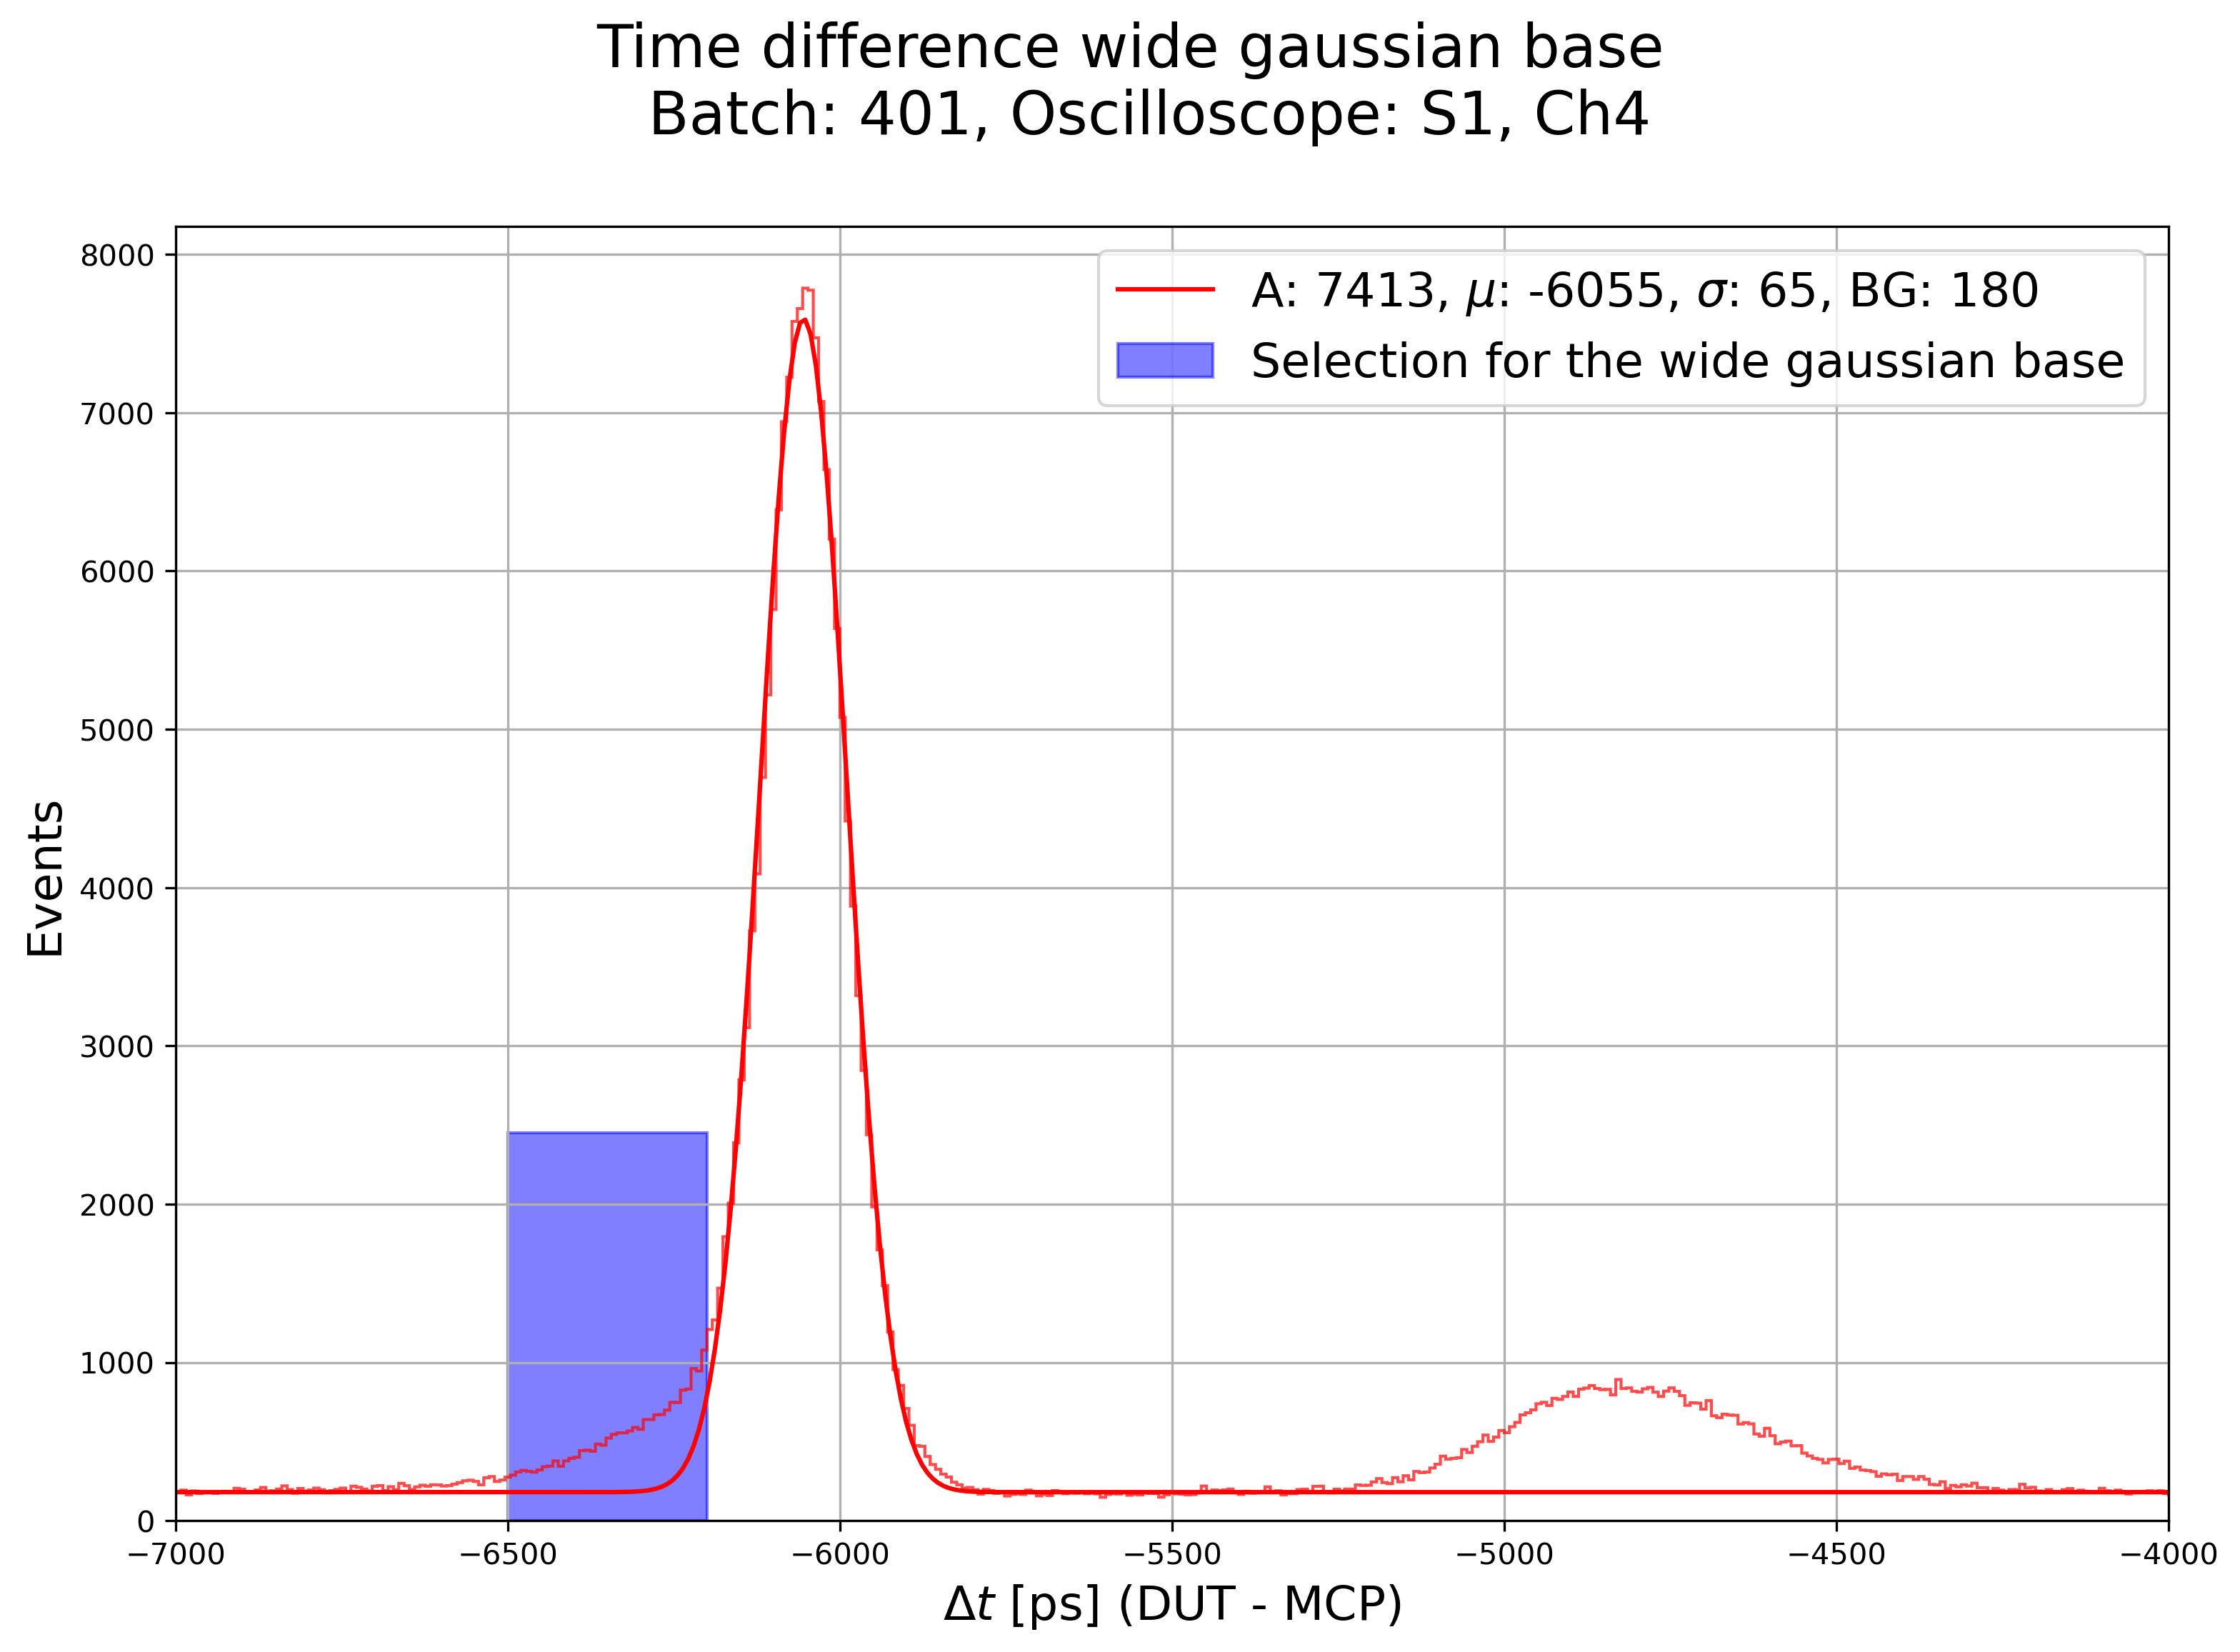
\includegraphics[width=.55\linewidth]{Images/detailed_analysis/time_difference_401_S1_dut_3_with_wide gaussian_left.png}
    \hfill
    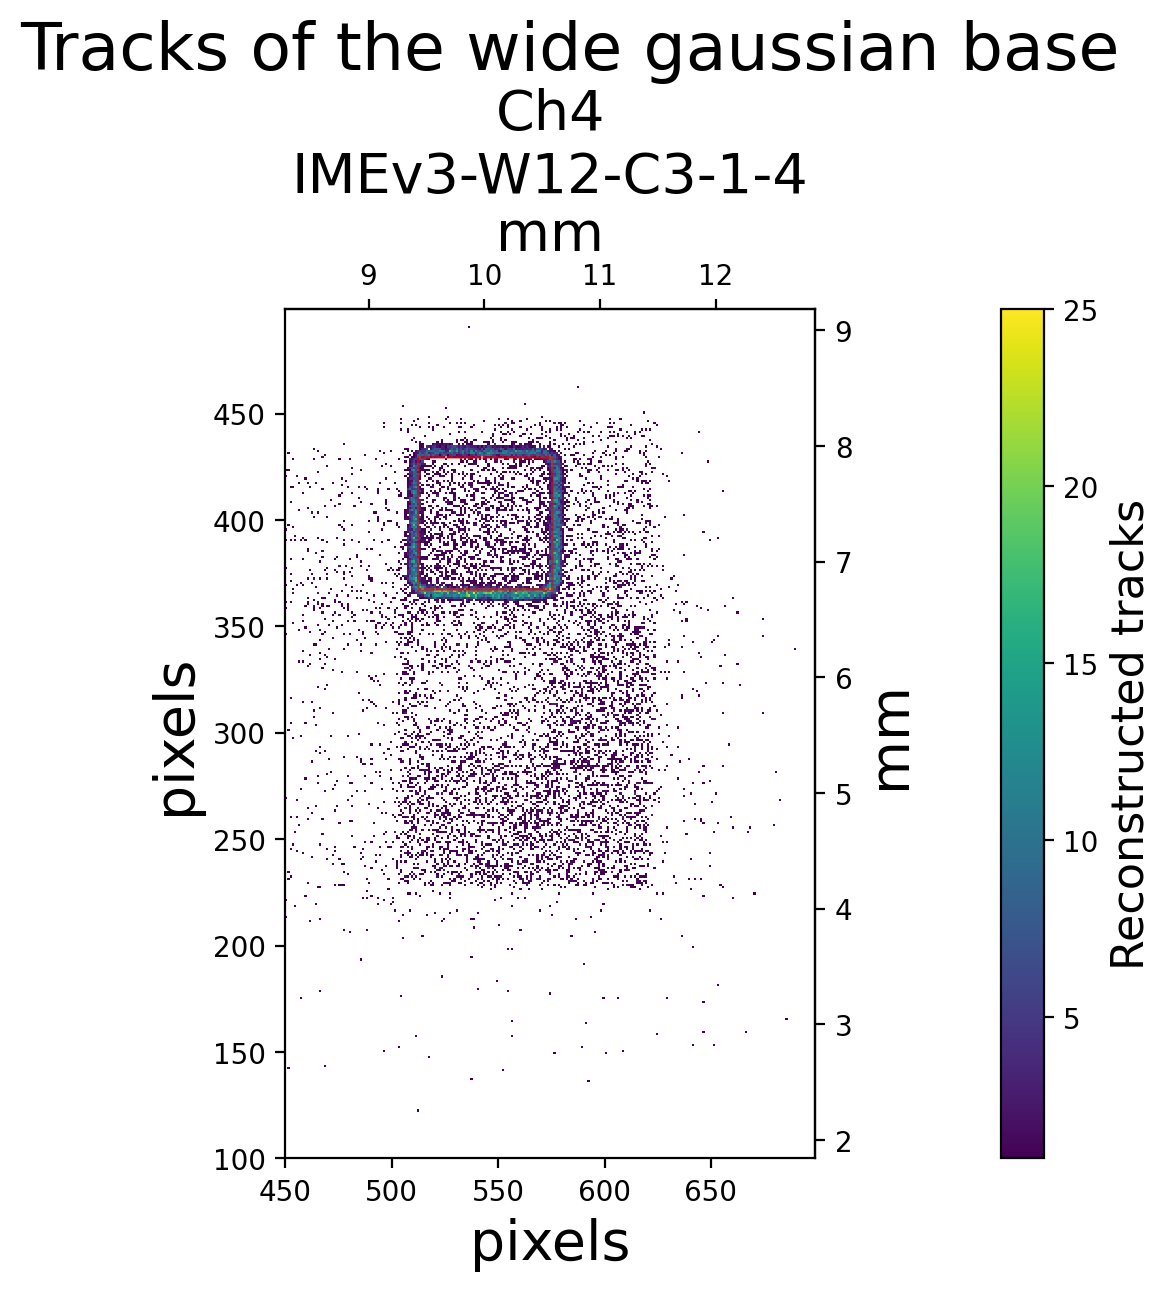
\includegraphics[width=.43\linewidth]{Images/detailed_analysis/2D Tracks 401_S1_dut_3_with_wide_gaussian_base_left.png}
    \captionsetup{width=\captionwidth}
    \caption{Left: selection of the "wide base" of the distribution. \\
    Right: tracks of events inside blue interva.l}
    \label{fig:time_difference_wide_gaussian}
\end{figure}


\subsection{Signal from neighbouring pads}\label{sec:multiple_peaks}

As it was very obvious from Figure \ref{fig:time_cut_gauss+bg_fit}, a second peak appeared in the time distribution.

By picking all the events in a certain time interval and plotting their corresponding reconstructed tracks, we were able to verify that: the main peak simply coincides with the DUT, the second peak arises from events picked up by its neighbouring pad. Figure \ref{fig:time_difference_multiple_peaks_highlight} is evidence of this.
As further confirmation this effect was only observed in DUTs which were part of 2\(\times\)2 LGAD arrays.

\begin{figure}[h!tbp]
    \centering
    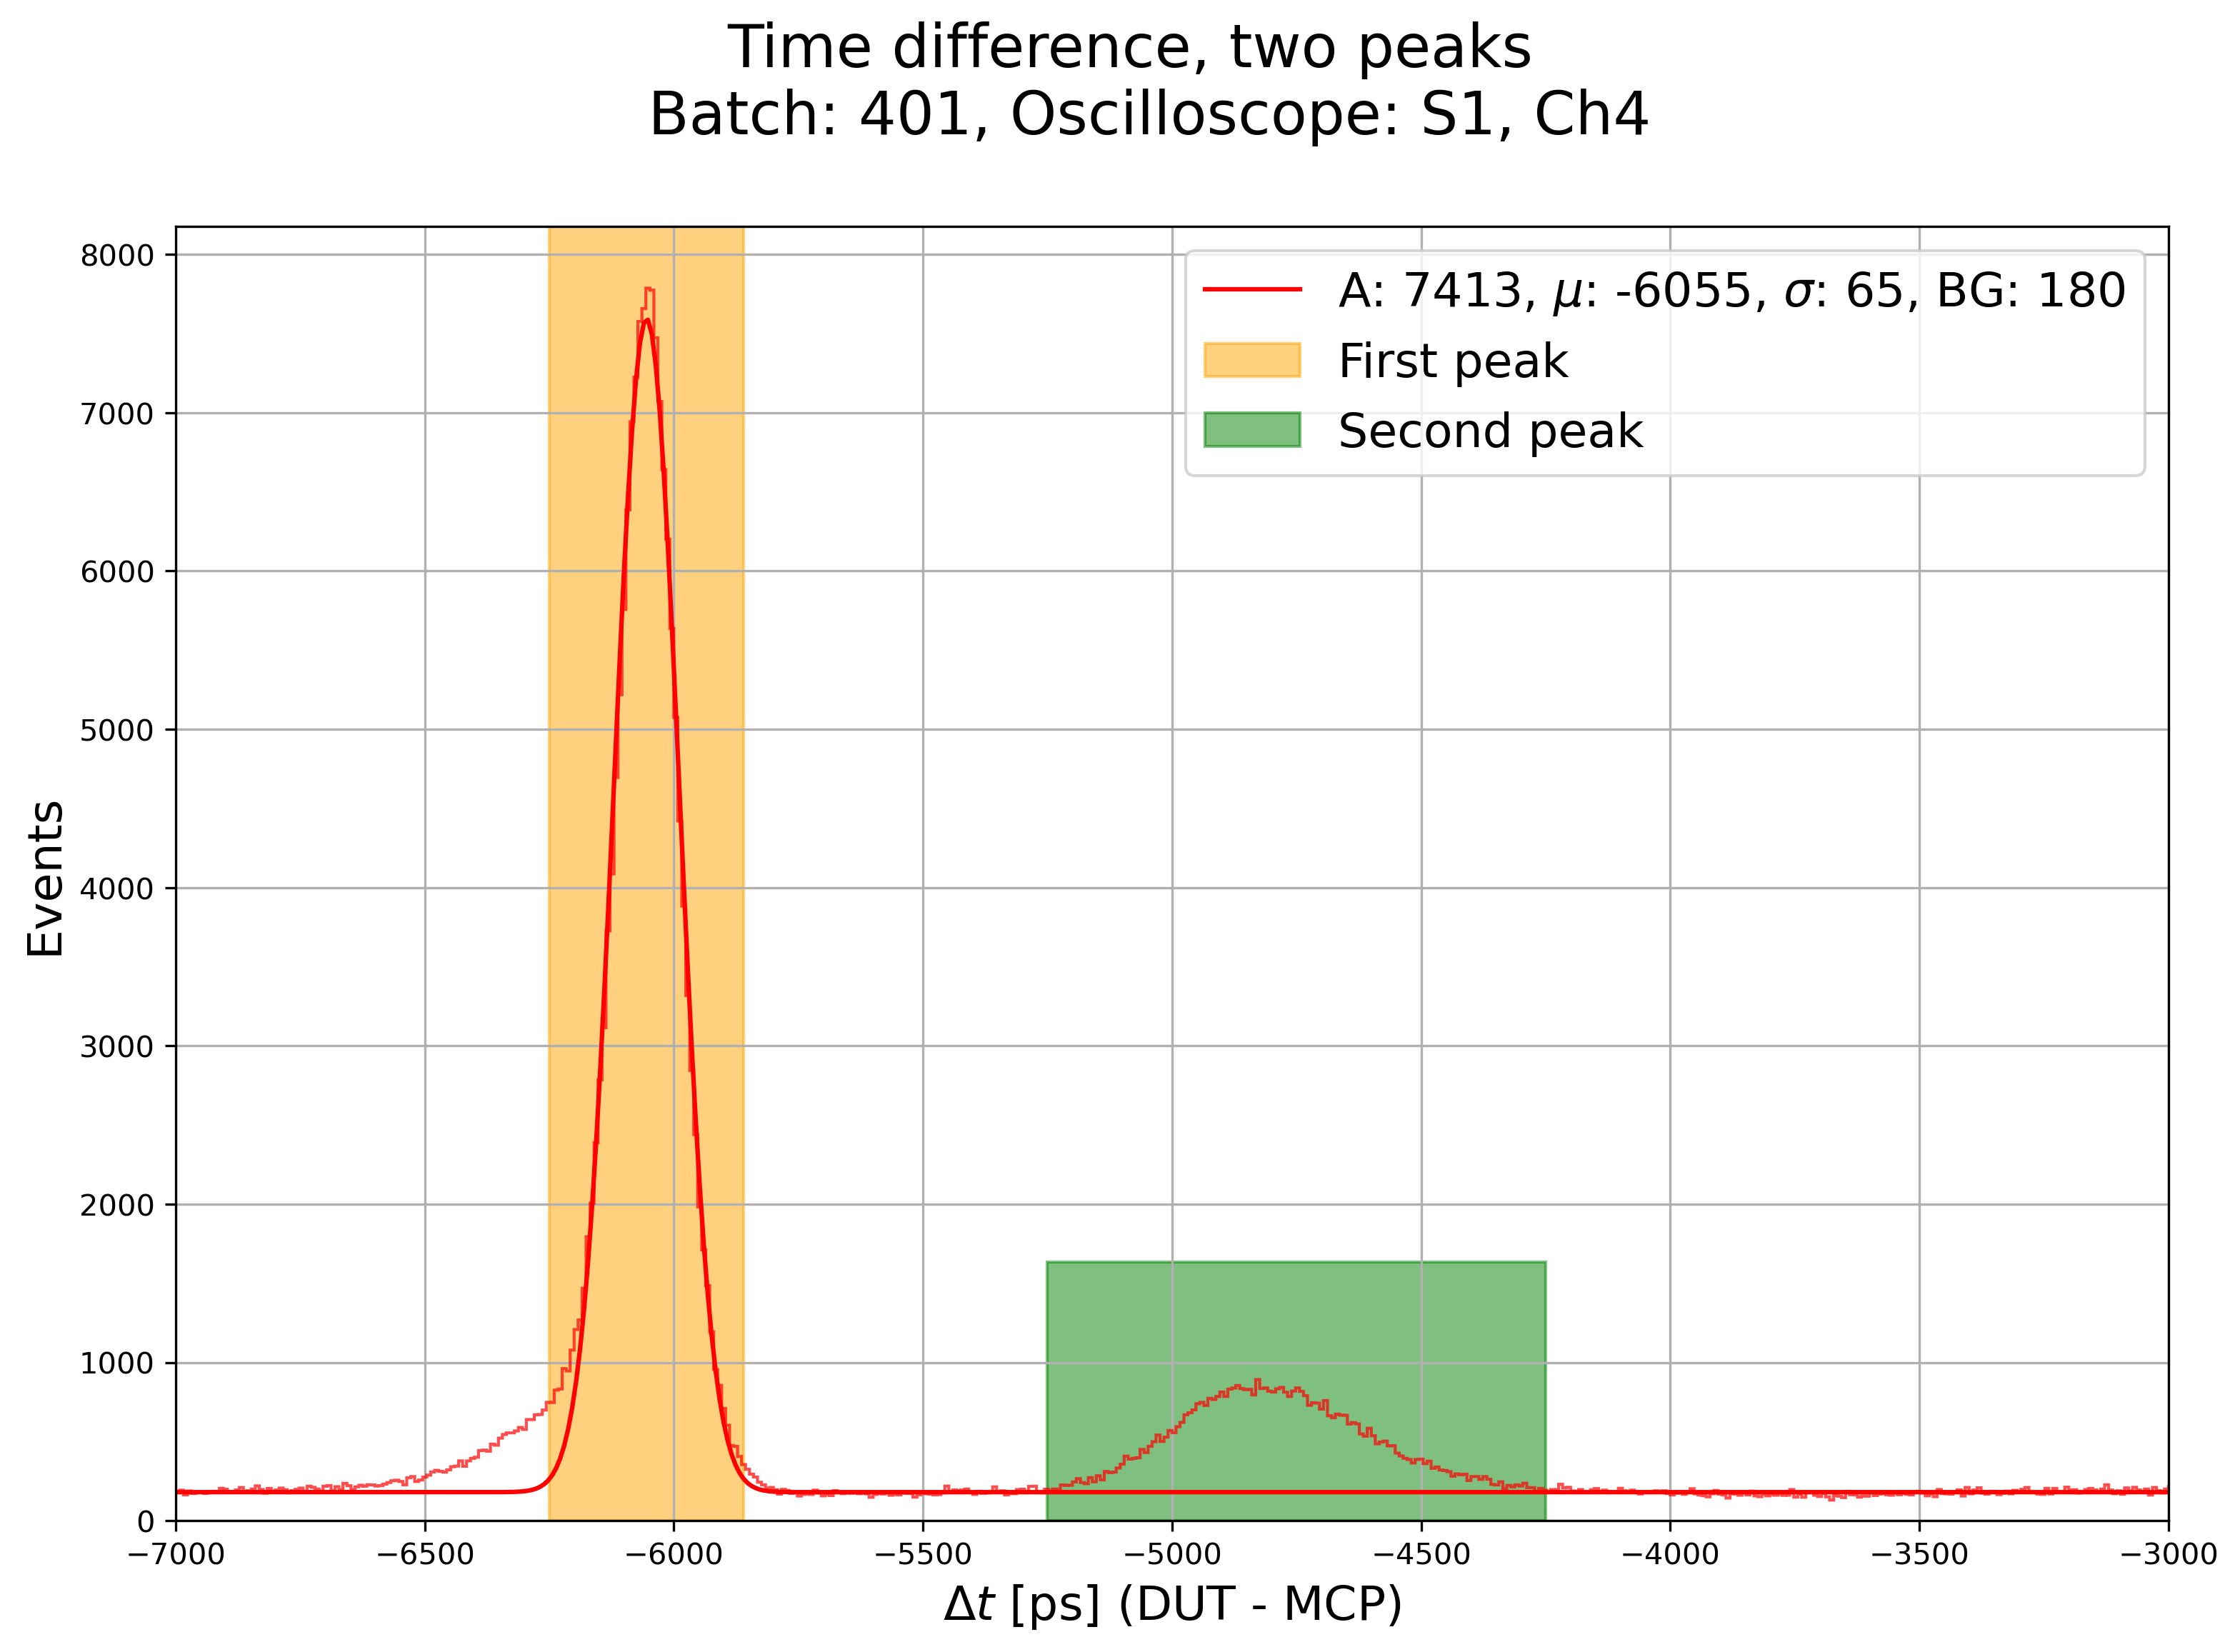
\includegraphics[width=.6\linewidth]{Images/detailed_analysis/time_difference_401_S1_dut_3_with_both_peaks_simple.png}
    \\ [\smallskipamount]
    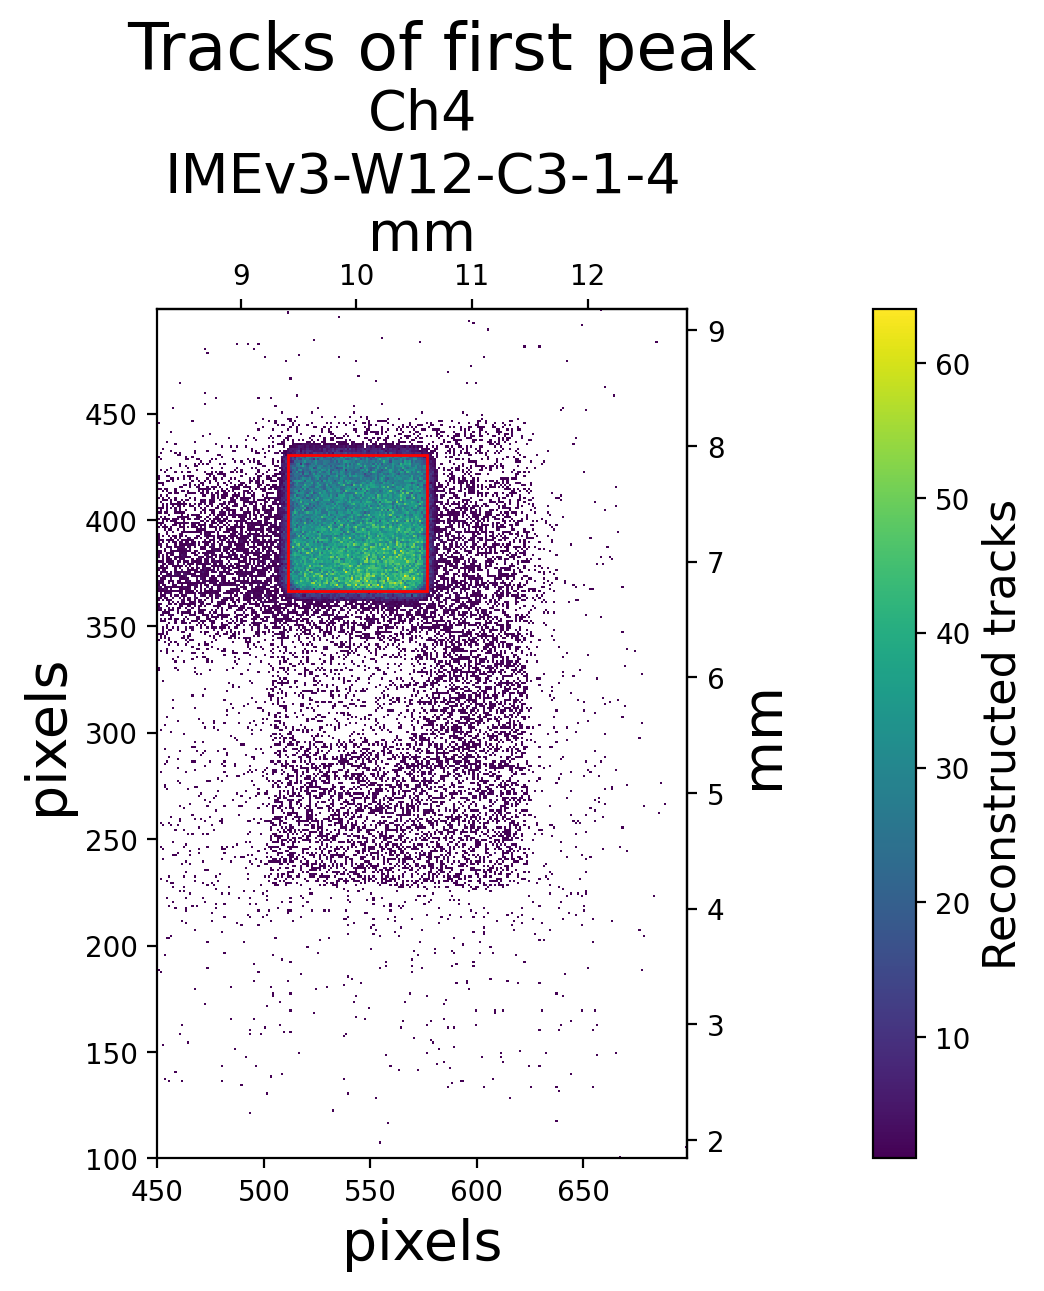
\includegraphics[width=.47\linewidth]{Images/detailed_analysis/2D Tracks 401_S1_dut_3_with_first_peak.png}
    \hfill
    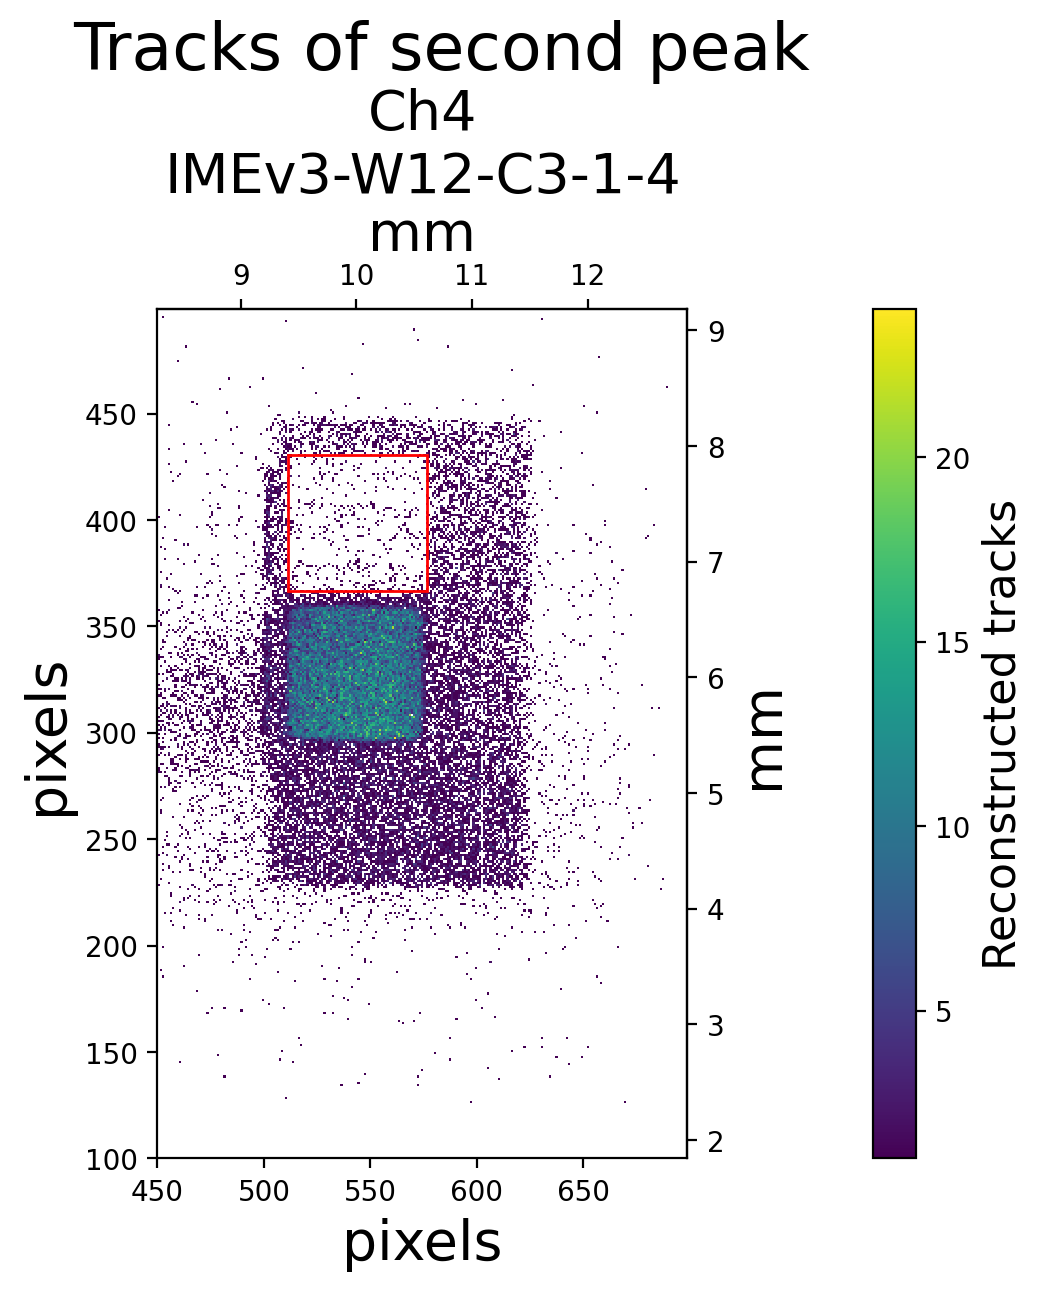
\includegraphics[width=.47\linewidth]{Images/detailed_analysis/2D Tracks 401_S1_dut_3_with_second_peak.png}
    \captionsetup{width=\captionwidth}
    \caption{Top: Time distribution with the first and second peak highlighted in yellow and green, respectively.
    Left: Tracks of events inside yellow interval.
    Right: Tracks of events inside green interval. In red is the outline of the DUT as estimated by the \textit{geometry cut} (\nameref{sec:geometry_cut}).}
    \label{fig:time_difference_multiple_peaks_highlight}
\end{figure}

\marginpar{\flushleft Separate the plots so that the text can fit better}

\FloatBarrier

\subsection{Pulse clipping}\label{sec:pulse_clipping}

As briefly mentioned before, there was indirect evidence that the pulses recorded by the oscilloscopes had been "cut" at their highest point. To prove this, the waveforms data was investigated, and a sample is shown in Figure \ref{fig:clipped_pulse}. The outcomes were:

\begin{itemize}
    \item Anomaly in the pulse height distribution (Figure \ref{fig:pulseHeight_cut})
    \item Irregularities in the charge distribution (Figure \ref{fig:charge_vs_pulseHeight_for_clipping})
\end{itemize}
Fortunately, this effect only impacted a small percentage of the data.

\begin{figure}[h!tbp]
    \centering
    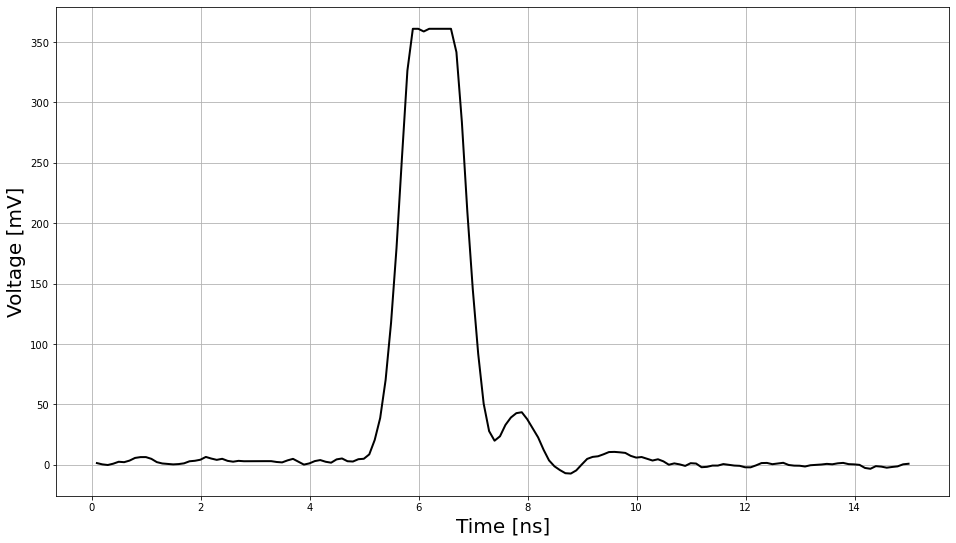
\includegraphics[width=.9\linewidth]{Images/detailed_analysis/Waveform of clipped pulse (ns).png}
    \captionsetup{width=\captionwidth}
    \caption{Example of a single pulse with the highest section cut out}
    \label{fig:clipped_pulse}
\end{figure}
 

\subsubsection{Discrepancies in the tail}\label{subsec:tail_discrepancies}
In a few cases the tail of the distribution deviated considerably from the expected function. We were able to successfully explain this discrepancy with the "clipping" effect in some pulses, due to the limit set to amplitudes registered by the oscilloscopes.
In Section \ref{sec:pulse_clipping} an example of a clipped pulse and its other aftereffects are shown.

In Figure \ref{fig:charge_vs_pulseHeight_for_clipping} (right) the pulse height is plotted against the charge and the clipped events appear very clearly at the rightmost part of the plot. This group of events overlapped with the expected charge distribution and could not be removed without modifying it. For this reason, the only solution was to adjust the range of the fit to try to exclude these events.

\begin{figure}[h!tbp]
    \centering
    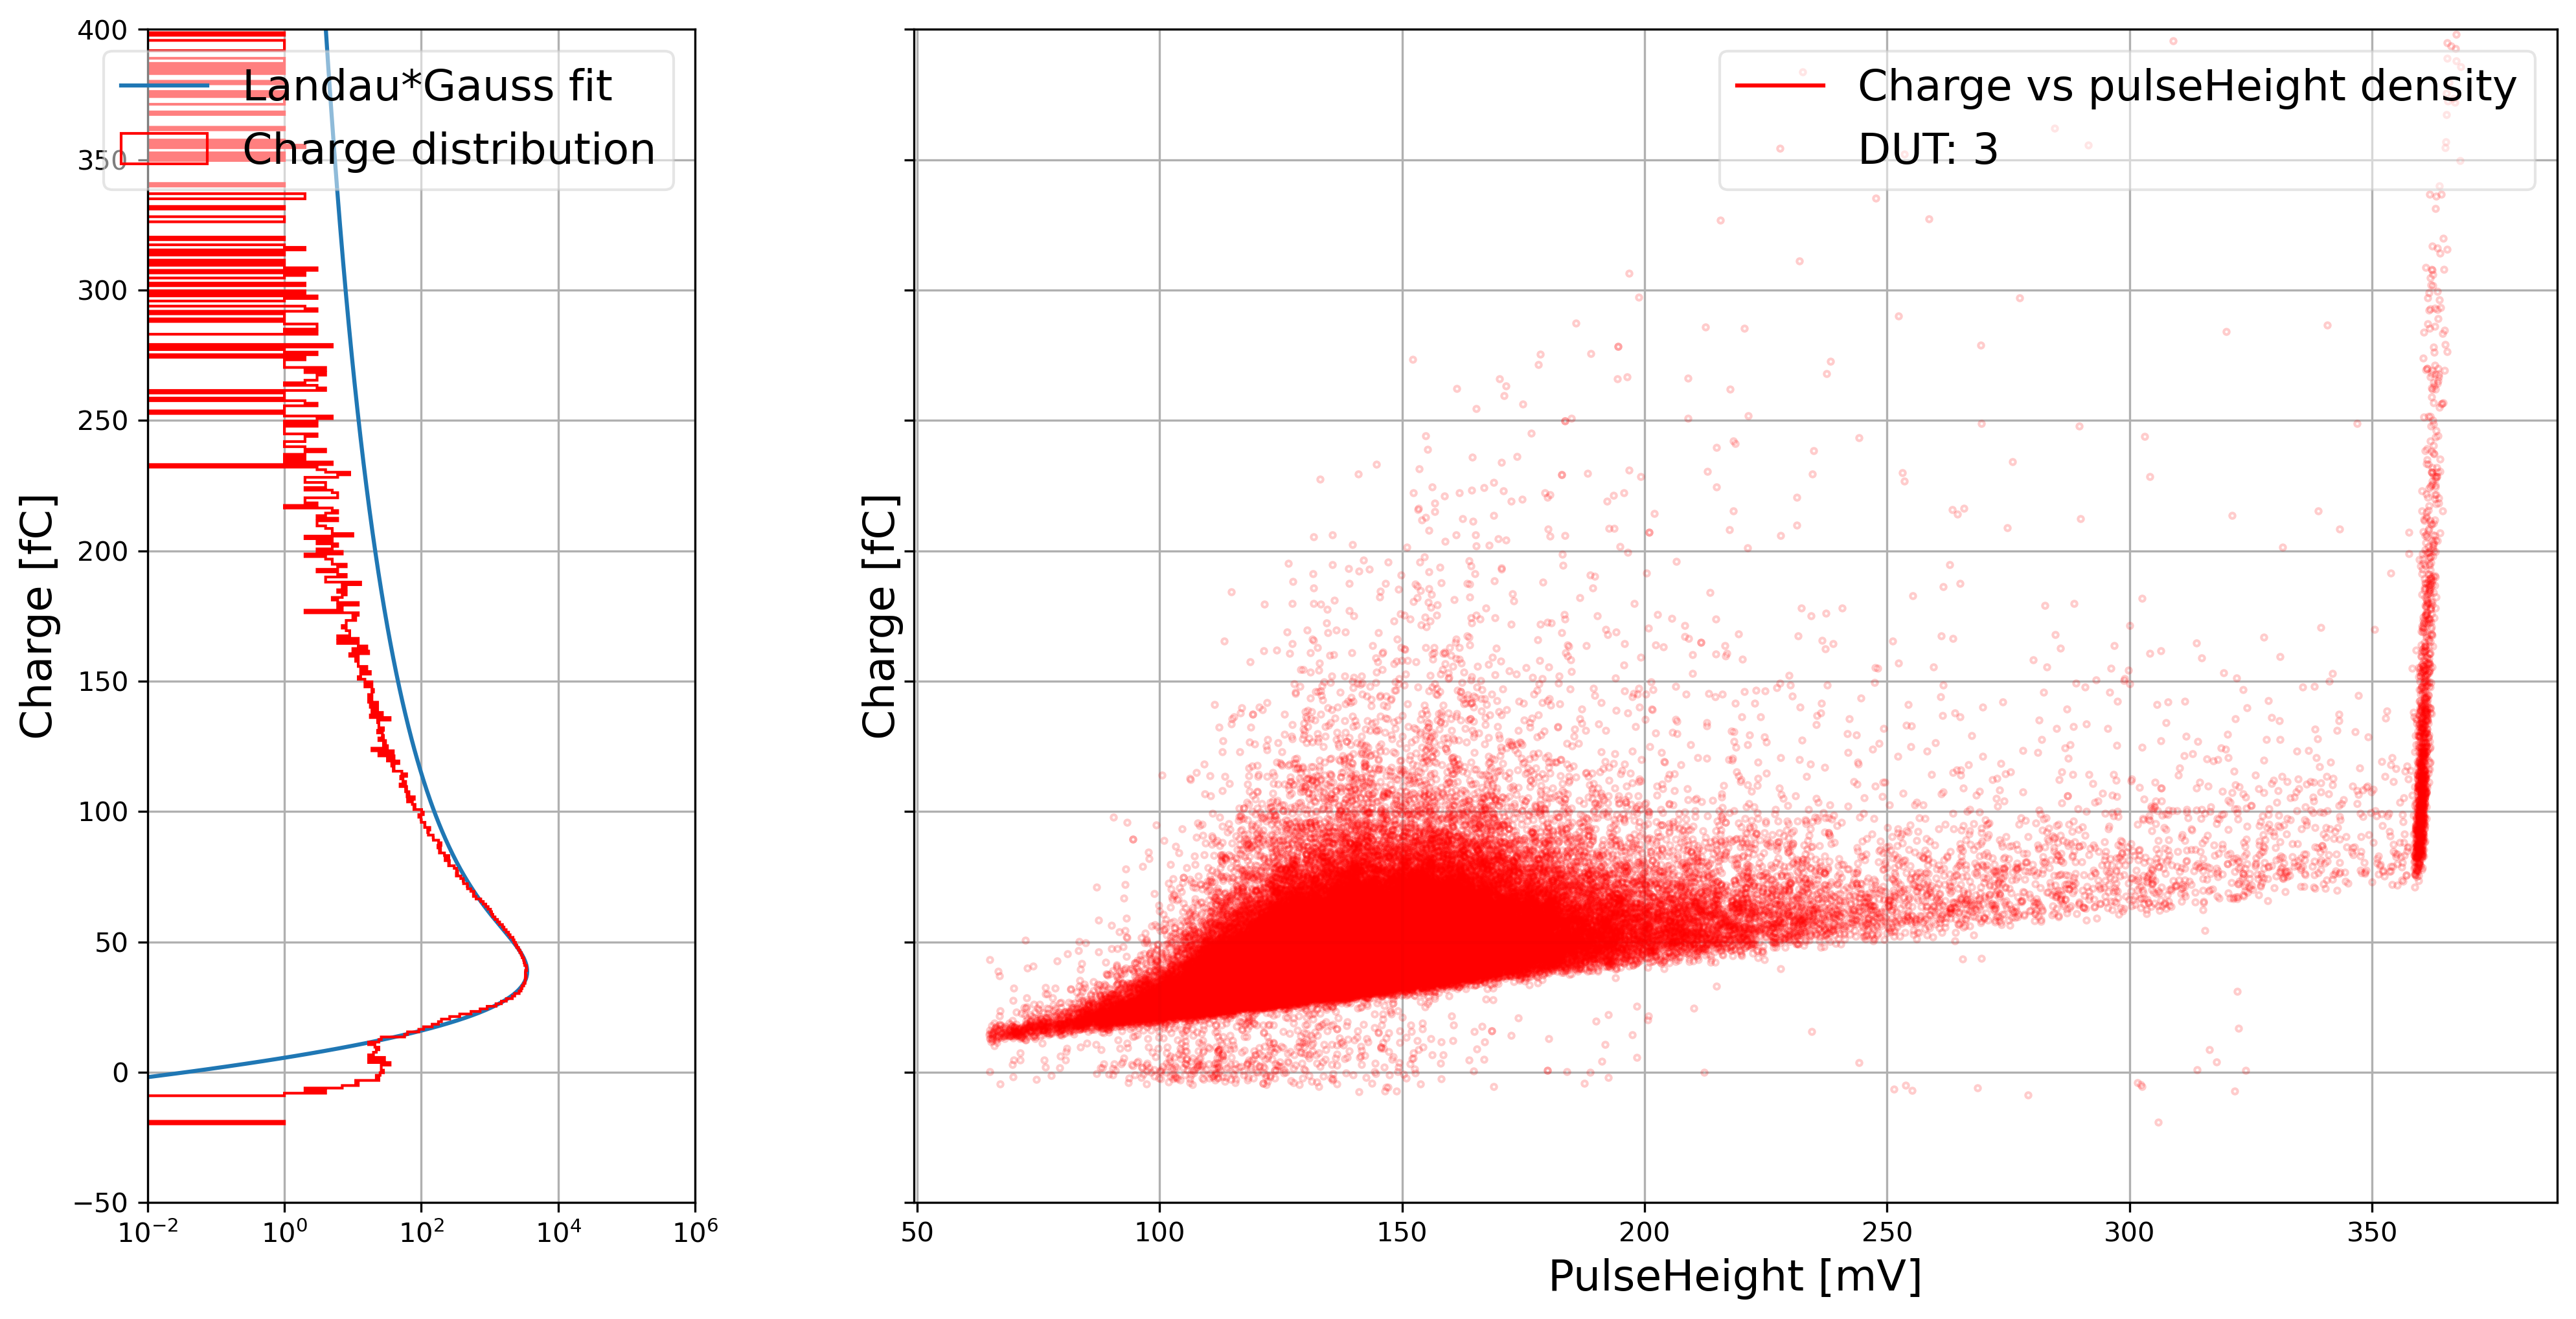
\includegraphics[width=1\linewidth]{Images/charge_plots/Charge_vs_pulseHeight_density_413_S2_dut3.png}
    \captionsetup{width=\captionwidth}
    \caption{Left: distribution of collected charge with Gaussian*Landau fit. Right: scatter plot Pulse height vs Charge, revealing the cause of the irregular tail}
    \label{fig:charge_vs_pulseHeight_for_clipping}
\end{figure}

\FloatBarrier

\subsection{Temperature fluctuations}\label{sec:temperature_fluctuations}

During the data taking there was a short malfunction of the cooling box containing the DUTs, which caused the temperature to rise up to \(\approx\qty{-26}{\degreeCelsius}\). The batch was excluded from the previous analysis, but it showed that the sensors have a significant sensitivity to temperature, so it was deemed interesting enough to report.

\begin{figure}[h!tbp]
    \centering
    \begin{minipage}[c]{.47\linewidth}
    \subfloat[Temperature vs Charge]{
        \includegraphics[width=.95\linewidth]{Images/Results/temperature fluctuations/Charge vs temperature 413_S1_dut[1, 2, 3].png}
        \label{fig:temperature_charge_S1}}
    \end{minipage}
    \hfill
    \begin{minipage}[c]{.47\linewidth}
    \subfloat[Temperature vs Time resolution]{
        \includegraphics[width=.95\linewidth]{Images/Results/temperature fluctuations/Time resolution vs temperature 413_S1_dut[1, 2, 3].png}
        \label{fig:temperature_time_res_S1}}
    \end{minipage}
    \vfill
    \begin{minipage}[c]{.47\linewidth}
        \subfloat[Temperature vs Charge]{
            \includegraphics[width=.95\linewidth]{Images/Results/temperature fluctuations/Charge vs temperature 413_S2_dut[1, 2, 3].png}
            \label{fig:temperature_charge_S2}}
        \end{minipage}
        \hfill
        \begin{minipage}[c]{.47\linewidth}
        \subfloat[Temperature vs Time resolution]{
            \includegraphics[width=.95\linewidth]{Images/Results/temperature fluctuations/Time resolution vs temperature 413_S2_dut[1, 2, 3].png}
            \label{fig:temperature_time_res_S2}}
        \end{minipage}
    
    \captionsetup{width=\captionwidth}
    \caption{Plots of the charge and the time resolution as function of the temperature, showing a clear dependence across all sensors. NB: The sensors shown here were operated at different voltages, so this plot is not meant to be a comparison between them, rather an observation of the general trend of each of them individually.}
\end{figure}

% \subsection{Charge sharing}\label{sec:charge_sharing}

\subsection{Interpad study}\label{sec:neighbouring_pads}
\begin{figure}[h!tbp]
    \centering
    \includegraphics[width=0.5\linewidth]{Images/detailed_analysis/batch 401 duts:3 and 3, edge efficiency studies.png}
    \captionsetup{width=\captionwidth}
    \caption{Efficiency projected onto one direction, measured between two neighbouring pads.}
    \label{fig:neighbouring_pads}
\end{figure}


\subsection{Charge sharing}

